\chapter{Conceptos básicos y metodología}



En un caso real, la planta generadora proporciona los valores de potencia que se introducen en cada modelo más el histórico que irá siendo almacenado. Debido a la falta de tiempo y recursos no se realizará la experimentación sobre una planta real, por ello en este trabajo simularemos con modelos de Simulink las plantas generadoras. 

En siguiente gráfico representa el proceso de generación de predicciones usado en el proyecto, desde las entradas hasta las salidas.

\begin{figure}[h]
    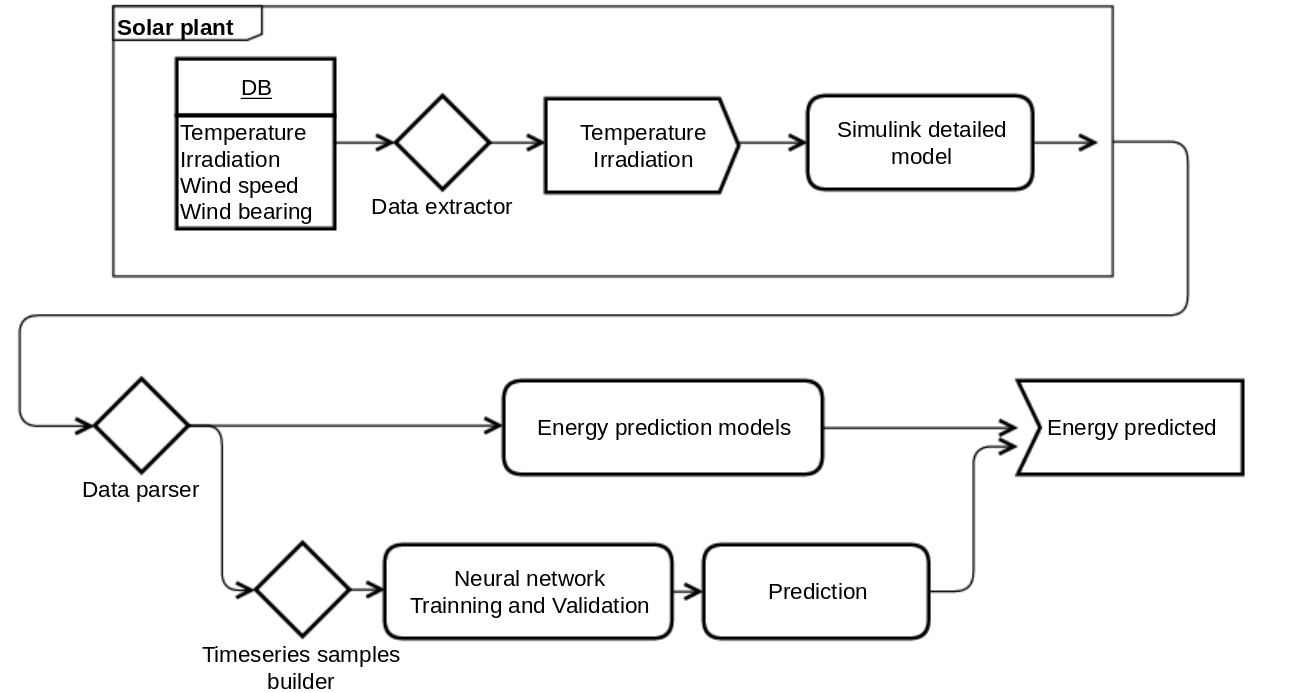
\includegraphics[width=\textwidth]{graphs/full-pipeline.png}
    \caption{Pipeline de predicción}
    \label{fig:full_pipeline}
\end{figure}

En el diagrama, la caja que contiene "Solar plant" representa lo que realmente sería una planta solar y que tiene como salida la "Potencia actual". Esta esta compuesta por:

\begin{itemize}
	\item La base de datos de donde extraeremos los valores de irradiación y temperatura, que hay sido previamente guardados para poder operar con ellos de manera mas cómoda, pero que realmente sería un valor continuo.
	\item El extractor de datos, cuyo propósito es extraer los datos de la base de datos, revisar la coherencia e integridad (En caso de que alguna entrada en la base de datos no exista o se haya borrado, la rellenará con coherencia) y darle un formato apto para Matlab.
	\item Finalmente el modelo detallado de Simulink junto con Matlab, procesarán las entradas y producirá una salida.
\end{itemize}

El siguiente paso ya sería la propia predicción: 

\begin{itemize}
	\item Primero se trata la salida de la planta (Esta será un valor continuo que habrá que discretizar y darle un formato de vector o matriz, de valores, celdas o muestras de series temporales).
	\item Posteriormente cada modelo realizará la predicción oportuna dando una salida y unas gráficas de rendimiento (Comparativas y error absoluto). 
\end{itemize}



\section{Predicción energética sobre pronostico} 
\label{sec:prediccion_energetica_sobre_pronostico}

El gran problema de las energías renovables es su falta de estabilidad y su complejo pronostico. En el caso de la energía solar, no habrá dos días que tengan la misma producción energética porque depende de la irradiación, de la temperatura, del angulo, la contaminación, etc. Aunque si se podrá exprimir la periodicidad del sol; En el caso de la energía eólica, el viento dependerá de la presión atmosférica, de la posición de las borrascas, la zona, la altura, etc.

Por esto, se dedicara el trabajo a las predicciones basadas en modelos auto-regresivos.
El resultado de la predicción será contrastado con los valores reales medidos del periodo precedido (Extraídos de la planta simulada).

Si por ejemplo queremos predecir el día siguiente, usaremos como histórico x días pasados y el resultado podremos contrastarlo con el valor real del día siguiente sin esperar a este por tener todos los valores ya guardados en la base de datos.

Otra duda que podría aparecer es "Por qué usar este modelo de predicción si se puede pronosticar el tiempo con muchísima mas exactitud?". Es cierto que la predicción en lo que respecta al clima está mucho mas avanzada, pero tener la predicción como entrada y la potencia como salida (A fin de contrastarla con la demandada) implicaría tener un modelo exacto de la planta generadora que permita obtener en función de las múltiples variables que afectadas, la potencia. Esto, aunque es una solución óptima, queda fuera del ámbito del proyecto ya que los pilares son los modelos auto-regresivos, los cuales se abstraen de los detalles técnicos. 

\section{Solar} 
\label{sec:solar}


\subsection{Modelos de predicción} 
\label{sub:modelos_de_prediccion}

Los modelos se expresan en términos de energía y tienen horizontes de predicción diferentes, horarios principalmente. Por esto, los modelos que tengan un horizonte de predicción de 1 hora, se mantendrán (No son capaces de proporcionar una predicción válida a 24 horas y modificarlos podría inducir a errores) y los que tengan un horizonte definido por el usuario (Red neuronal, N4SID o ARMA) se establecerán a 24 horas. 

La predicción de energía solar se abordará con los siguientes modelos:
\begin{itemize}
	\item Exponentially weighted moving average
	\item Predictor for adaptive management developed at ETHZ
	\item Optimal 2D linar prediction filter
	\item Exponentially Weighted Moving Average
	\item Exponentially Weighted Moving Average with Phase Displacement Regulator
	\item Neural network
	\item N4SID
\end{itemize}


\subsubsection{ Exponentially weighted moving average } 
\label{ssub:subsubsection_name}

El modelo Exponentially Weighted Moving Average (EWMA \cite{ewma}) es el mas sencillo y tradicional. Para poder ajustarse al ciclo solar, se realizan subsegmentos de tamaño \textbf{numero de muestras por dia}. 
Este se basa en una suma basculada de los valores Real y Pronosticado, siendo este ultimo el resultado del pronostico del día anterior.

\begin{align}
	E_{PRED}(d+1) &= \rho E_{REAL}(d) + (1-\rho) E_{PRED}(d)
\end{align}

La energía pronosticada en un momento t y día d sera la suma de la energía medida en el momento t del día anterior y la energía pronosticada en el momento t del día anterior.

En esencia, el algoritmo usa el histórico de los días anteriores para predecir el siguiente. Si la constante $\rho$ esta mas cerca del 1, el pronostico tendera a ser el valor del día anterior. Sin embargo, si $\rho$ es mas próxima al 0, se explotara el registro acumulado. 

Pros: Bajo procesamiento y consumo de memoria

Cons: Predicción muy simple sin control de errores


\subsubsection{ Predictor for adaptive management developed at ETHZ } 
\label{ssub:subsubsection_name}

Este modelo \cite{ethz} de predicción combina la predicción a corto plazo (horas) con largo plazo (días).

\begin{align}
	E_S(t) &= min( (1-\gamma) E_N(t) + (\gamma) R(t), E_N(t) ) \\
	R(t) &= \beta R(t-1) + (1-\beta) E_S(t-1) \\
	E_N(t) &= \alpha E_N(t-1) + (1-\alpha) E_S(t-1)
\end{align}

$E_S$ es la energía real producida por la planta fotovoltaica,\\
$E_N$ es la energía promedio medida en T ultimas muestras con factor $\alpha$
Finalmente R es el promedio a corto plazo con factor $\beta$

Este algoritmo se basa en el mismo principio que el EWMA separando el corto plazo del largo plazo.

Pros: Tiene mejor factor de predicción a corto plazo que el EWMA

Cons: Sigue sin filtrar variaciones habituales y no es inmune a imprevistos


\subsubsection{ Optimal 2D linar prediction filter } 
\label{ssub:subsubsection_name}

El fundamento de este algoritmo \cite{o2d} es la representación matricial de la energía. Siendo las filas los días y las columnas los momentos (horas en el estudio) ambas ordenadas en orden creciente, un nuevo dato de energía es igual a los valores de la columna (K días anteriores) mas los valores de fila (K horas anteriores) mas los valores previos $((K-1)^2$ horas anteriores en días anteriores).

Siendo el tamaño de venta K y el nuevo valor $(K,K)$, los valores $(\_,K-1)$ son los días, $(K-1,\_)$ son las horas y $([1,K-1],[1,K-1])$ son los valores previos no relacionados. 

Cada uno de estos 3 elementos sera multiplicado por unos coeficientes a1, a2 y a3. 

Este seria un ejemplo para tamaño de ventana K = 2

\begin{align}
	X'_{i+1,j+1} &= a_1 X_{i,j} + a_2 X_{i,j+1} + a_3 X_{i+1,j}
\end{align}

Para tamaño de ventana superior simplemente sumar la columna multiplicada por $a_1$ y dividida por K. Lo mismo con la fila y con la submatriz que queda de quitar la fila y columna.

Pros: Toma valores del histórico para

Cons: Igual que EWMA o ETHZ, no tiene control de errores ni modifica las variables dinamicamente.


\subsubsection{ Weather Conditioned Moving Average} 
\label{ssub:subsubsection_name}

El algoritmo mas explotado en la literatura, WCMA \cite{ewma}, tiene sus bases en el EWMA con el valor añadido de que tiene una visión global del periodo y control de cambios.

\begin{align}
	E_{(d,n+1)} &= \alpha E_{(d,n)} + (1-\alpha) \frac  {\sum_{i=1}^D E_{i,n+1}} {D} \\
	v^{d,n}_k &= E_{(d,n-k+1)} \frac {D}{\sum^D_i=1} E_{i,n-k+1} \\
	p_k &= 1-\frac {K-k+1}{K} \\
	GAP_k^{d,n} &= V^{d,n}(K) \times \big(P(K) / \sum P(K) \big)^T \\
	E^{GAP}_{d,n+1} &= \alpha E_(d,n) + (1-\alpha) GAP_K^{d,n} \frac{\sum^D_{i=1} E_{i,n+1}}{D}
\end{align}

$E_{(d,n+1)}$ esta es la energía calculada siguiendo el mismo estilo que EWMA. 

Con $v^{d,n}_k$ se obtiene la mejora de las condiciones a lo largo de un periodo k previamente definido. Si v > 1 se considera que las condiciones del momento n del dia d son mejores que los días anteriores. Iguales o peores en otro caso.

$p_k$ es un vector de longitud k cuyo objetivo es dar mas importancia a los valores mas cercanos al momento actual. Esto se consigue con un vector creciente entre 0 y 1 que representa una recta creciente. e.g. [0, 0.33, 0.66, 1]

$GAP_k^{d,n}$ es el valor clave del algoritmo. Como se ve en la fórmula, contiene V y P. De esto se concluye que GAP representa la cantidad de energía de más o de menos que hay actualmente, ya que compara el momento actual con los valores anteriores, cuantificados con P (valor más cercano al actual, mas peso) dando como resultado > 1 si hay más energía disponible o < 1 si hay menos.

Finalmente $E^{GAP}_{d,n+1}$ es el resultado de la predicción.


Pros: Permite tener constancia de los cambios mas recientes gracias a la $v^{d,n}_k$

Cons: Si no se tiene control de posibles valores negativos ()


\subsubsection{ Weather Conditioned Moving Average with Phase Displacement Regulator} 
\label{ssub:subsubsection_name}

Esta mejora del algoritmo WCMA incluye la variable PDR que permite seguir el rastro de los errores además de reajustarlos. Esto se realiza gracias al histórico de errores. En función de el error que se observó en ese momento de días, se suma o resta el error a fin de neutralizarlo. 

\begin{align}
	PE(d,i) &= \delta PE(d-1,i) + (1-\delta) \frac  {\sum_{i=1}^D PE_{i,n+1}} {D} \\
	PDR_{d,n} &= \bigg[ \frac{\sum^{w-1}_{w_i = 0} [ PE(n-w_i) + PE(n+w_i) ] \gamma^{(w_i + 1)}}{\sum_{w_i = 0}^{w - 1} \gamma^{(w_i + 1)}} \bigg] \\
	E^{PDR}_(d,n+1) &= \alpha E_{d,n} + (1-\alpha ) GAP^{d,n}_K \frac{\sum^D_{d,n} E_{i,n+1} }{D} + PDR_{d,n+1}
\end{align}

$PE(d,i)$ representa el error en cada momento, basculado con los errores pasados.

$PDR_{d,n}$ es el valor final que regula la salida del algoritmo. Toma como valor clave PE, más concretamente, un PE con tamaño de venta 2w (los w PE anteriores y w PE siguientes). Esto permite equilibrar el error entre los que le rodean. 

Pros: Tiene control del error pasado

Cons: Necesita un registro importante de valores para ajustarse bien


\subsubsection{ Neural network prediction} 
\label{ssub:subsubsection_name}

Consideraremos también una red neuronal. Estas al estas destinadas a resolver problemas cuyas entradas están fuera de lo esperado hacen aparentemente idónea la solución ya que la variabilidad de las entradas (el clima) depende de muchas variables difíciles de contemplar simultáneamente.
Aprovecharemos la capacidad adaptativa y analítica con propagación hacia atrás para predecir valores con bajo coste de memoria.

La red neuronal estará diseñada con 2 capas de 4 neuronas y función sigmoidal $O = \frac{1}{(1+e^{-n})}$

El formato de entradas será el siguiente:
\begin{itemize}
	\item D entradas con los valores de los valores anteriores
	\item K entradas con los valores de los días anteriores
	\item K-1 entradas con las diferencias entre los días anteriores
\end{itemize}

El entrenamiento sera con el algoritmo de regularización Bayesiana, que mejorara el rendimiento con ruido, y con propagación hacia atrás, asi que las salidas conectaran con las salidas.

Pros: Puede reaccionar y predecir mejor ante situaciones inesperadas

Cons: Requiere un entrenamiento continuo. Consume muchos recursos


\subsubsection{N4SID}
\label{ssub:n4sid}

Este algoritmo (Sistema de identificación de subespacios de espacios de estados) permite estimar un modelo de espacio de estados usando subespacios.

Un modelo de espacio de estados es un modelo que usa variables de estado para describir un sistema con un sistema de ecuaciones diferenciales de primer orden o ecuaciones diferenciales. 

Los modelos de espacio de estados son apropiados para realizar estimaciones (predicciones en este caso) ya que solo requieren del orden, el cual esta relacionado con el retardo de las entradas y salidas a usar en la ecuación diferencial.

La representación del modelo estimado es un sistema como:

\begin{align}
	x(t) = Ax(t) + Bu(t) + Ke(t) \\
	y(t) = Cx(t) + Du(t) + d(t)
\end{align}

Donde A,B,C y D son matrices del espacio de estados, K es la matriz de perturbaciones, $u(t)$ es la entrada, $y(t)$ es la salida, $e(t)$ es la perturbación y $x(t)$ es el vector de nx estados, con nx igual al orden.



\subsection{Conclusiones} 
\label{sub:conclusiones}

A nivel de calidad de predicción cualquiera de las opciones que exploten tanto el histórico a largo plazo (Días) como a corto plazo (momentos anteriores) y tenga en cuenta el peso de la proximidad de los valores, es una buena opción de predictor de serie temporal.

De estos modelos se puede extraer que los más favorables son el EWMA y el EWMA con PDR. Queda excluida la red neuronal debido a su excesivo tiempo de entrenamiento y predicción. 




\section{Eolica} 
\label{sec:eolica}

\subsection{Modelos de predicción} 
\label{sub:coneptos_basicos}

La predicción de energía eólica es mucho mas compleja que la solar ya que la irradiación a lo largo del día sigue una distribución normal. Luego se verá afectada por múltiples factores como nubes o polución, pero el sol siempre sigue el mismo patrón. El viento, en cambio, no. Y esto dificulta mucho la tarea.

Abordaremos la predicción de energía eólica con los siguientes 2 modelos:
\begin{itemize}
	\item Modelo ARIMA
	\item N4SID
\end{itemize}


\subsubsection{ARMA/ARIMA}
\label{ssub:arima}

ARIMA: AutoRegressive Integrated Moving Average. Este modelo se usa, o para predecir valores (Su propósito aquí) o bien para entender los valores pasados.

Para entender un poco como funcionan los modelos ARIMA lo explicaremos por componentes.

El factor AutoRegressive, Auto regresivo o el AR de ARIMA define la variable en cualquier instante del tiempo como una combinación de los valores anteriores más un error.

El factor Moving Average, Media móvil o el MA de ARIMA define un valor de la variable como una suma de un valor $\alpha$ mas la suma ponderada de los errores.

El factor Integration o la I de ARIMA indica que un valor de la variable es la diferencia entre un valor y su sucesor, pudiendo haber sido realizada la diferencia varias veces.

Sabiendo esto el modelo ARIMA se enuncia como ARIMA(p,d,q) siendo p,d y q números naturales que representan la distancia del retardo a usar, el numero de veces que se realizó la resta en la diferencia y el orden de la ecuación de media móvil.